\section{Heur\'istica Constructiva Golosa} \label{ej3}
\subsection{Explicaci\'on}
La heurística constructiva golosa busca, dado un grafo, determinar un Conjunto Independiente Dominante Mínimo, eligiendo en cada iteraci\'on, la mejor opci\'on seg\'un el criterio definido\\

Nuestro criterio se basa en el grado de los nodos. Dado que el grafo nunca se modifica, podemos ordenar un conjunto con todos los nodos del grafo en funci\'on de su grado al comienzo del algoritmo.\\

Luego, haremos un ciclo iterando este conjunto, el primer nodo siempre ser\'a agregado al conjunto soluci\'on, y luego se procede a eliminarlo junto a sus vecinos.

Esto se traduce en elegir en cada paso el nodo de mayor grado que a\'un no haya sido dominado por otro con grado superior.\\

De esta manera, el algoritmo siempre obtiene un conjunto independiente (dado que por cada nodo que toma, elimina a sus vecinos) y dominante (dado que por cada nodo que toma, lo agrega al conjunto, y elimina a sus vecinos, es decir, que estos son adyacentes a un nodo del conjunto), pero no puede asegurar que siempre sea mínimo. Eso dependerá del grafo.\\

\begin{algorithm}[h!]
\caption{heur\'istica greedy}
vector$<$nodoGrado$>$grados(adyacencia.cantNodos());\\
\For{\textit{int} i = 0; i$ < $grados.size(); ++i\\}{
	grados[i].nodo = i;\\
	grados[i].grado = adyacencia.gradoDeNodo(i);
}
sort(grados.begin(), grados.end());\\
\While{grados.size()$ > $0}{
	\textit{unsigned int} nodo = grados[0].nodo;\\
	optimo.push_back(nodo);\\
	\textit{vector$<$nodoGrado$>$::iterator} iter = grados.begin();\\
	\While{iter != grados.end()}{
		\eIf{adyacencia.sonVecinos(nodo, iter-$>$nodo) or nodo == iter-$>$nodo}
			{iter = grados.erase(iter);}
			{iter++;	}
	}
}
\end{algorithm}

%Explicar detalladamente el algoritmo implementado.

\newpage
\subsection{Complejidad Temporal}\label{compej3}
En lo que respecta a la complejidad temporal, demostraremos a continuación que la misma es $O(n^{2})$, con n la cantidad de nodos del grafo.\\

Recordemos que el algoritmo ordena los nodos de mayor grado a menor grado, luego toma el primero de dicha lista, lo agrega al conjunto solución, y lo elimina de la lista junto a sus adyacentes. Luego repite el proceso, tomando el siguiente nodo de la lista de nodos restantes.\\

Dicho esto, definiremos a $f(i,n): \mathbb{N} \rightarrow \mathbb{N}$ como:\\

$f(i,n)$ = Cantidad de operaciones en el peor caso, teniendo $n$ nodos totales y faltando eliminar $i$.\\

Es decir,\par

\begin{itemize}
	\item$f(0,n) = c$, dado que no falta eliminar ningun nodo, el algoritmo termina, con $c$ alguna cantidad constante de operaciones.\par
	\item $(\forall i \in {1...n-1}) f(i,n) = h*(i-1) + f(i-1,n) + c$, con $h$ la cantidad de vecinos del nodo que estoy viendo, $c$ alguna cantidad constante de operaciones, y $f(i-1,n)$ es el llamado recursivo.
\end{itemize}

Expliquemos que significa cada monomio:
\begin{itemize}
	\item $h*(i-1)$: En el peor de los casos, recorre por cada nodo de la lista de adyacencia del nodo tomado, a los demas nodos sin marcar (sin incluir el nodo tomado).
	\item $f(i-1,n)$: En el peor de los casos, no hay nodos de la lista de adyacencia, que no hayan sido eliminados aún.
	\item $c$: Alguna cantidad constante de operaciones.
\end{itemize}

Entonces, querremos demostrar que $(\forall i \in {1...n-1}) f(i,n) \leq k*i*n + c$ (con $k$ y $c$ alguna constante), pues al momento de ejecutar el algoritmo, se tienen $n$ nodos, y faltan eliminar $n$ nodos, siendo la complejidad del mismo, $O(f(n,n)) = O(n^{2})$; y dado que la cantidad de nodos por borrar no puede ser mayor que la cantidad total de nodos, es correcto pedir que $0 \leq i < n$.\\

\newpage
{\large\textbf{Teorema}}\\

Dado $f(i,n): \mathbb{N} \rightarrow \mathbb{N}$ definida como\\

$f(i,n)$ = Cantidad de operaciones  en el peor caso, teniendo $n$ nodos totales y faltando eliminar $i$.\\

$f(0,n) = c$\\

$f(i,n) = h*(i-1) + f(i-1,n) + c$\\

Luego, $(\forall i \in {1...n-1}) f(i,n) \leq k*i*n + c$.\\

{\large\textbf{Demostración}}\\

Sea $P(i) = f(i,n) \leq k*i*n + c$, demostraremos por inducción global, que $(\forall i \in {1...n-1}) P(i)$\\

Entonces,\\

\textbf{Casos base:}

\begin{itemize}
    \item[•] $f(0,n) = c$
    \item[•] $f(1,n) = h*(1-1) + c = c \leq k*1*n + c$\\
    Dado que tengo $n$ nodos, y solo falta eliminar uno. $k$ es alguna cantidad constante de operaciones para eliminar el nodo y finalizar el algoritmo.
\end{itemize}

\textbf{Paso inductivo:}\\

$\underbrace{P(1) \wedge P(2) \wedge ... \wedge P(m-1)}_{\text{Hipótesis inductiva}} \Rightarrow \underbrace{P(m)}_{\text{Tesis inductiva}}$\\

Es decir, que por hipótesis inductiva, podemos suponer que vale $f(r,n) \leq k*r*n + c$, con $r \leq m-1$, y queremos ver que $f(m,n) \leq k*m*n + c$.\\

Luego,

\begin{align*}
f(m,n) & = h*(m-1) + f(m-1,n) + c \\
 \stackrel{HI}{\Longrightarrow} f(m,n) & \leq h*(m-1) + n*(m-1) + c \\
 \intertext{Dado que la cantidad de vecinos adyacentes esta acotada por la cantidad de nodos totales, $0 \leq h < n$, luego}
 & \leq n*(m-1)+n*(m-1) + c\\
 & \leq n*m + n*m + c\\
 & = 2*n*m + c\\
 & \leq \underbrace{k*n*m + c}_{\text{Tesis inductiva}} \text{       En particular, con $k = 2$ en este caso}
\end{align*}
\hfill $\blacksquare$

Entonces, $f(i,n) \leq c*i*n + k$, para algún $c$ y $k$ constantes.
Dado que el algoritmo ejecuta, en peor caso, $f(n,n)$ operaciones, su complejidad esta acotada por $f(n,n)$, por lo tanto, tiene complejidad $O(n^{2})$.\\

%Calcular el orden de complejidad temporal de peor caso del algoritmo.
\subsection{Comparaci\'on de resultados con soluci\'on \'optima}
La heurística constructiva golosa fallará en encontrar siempre la solución óptima.
Particularmente, existen grafos para los cuales la heurística fallará siempre.\\
  \begin{figure}[h!]
   \begin{center}
 	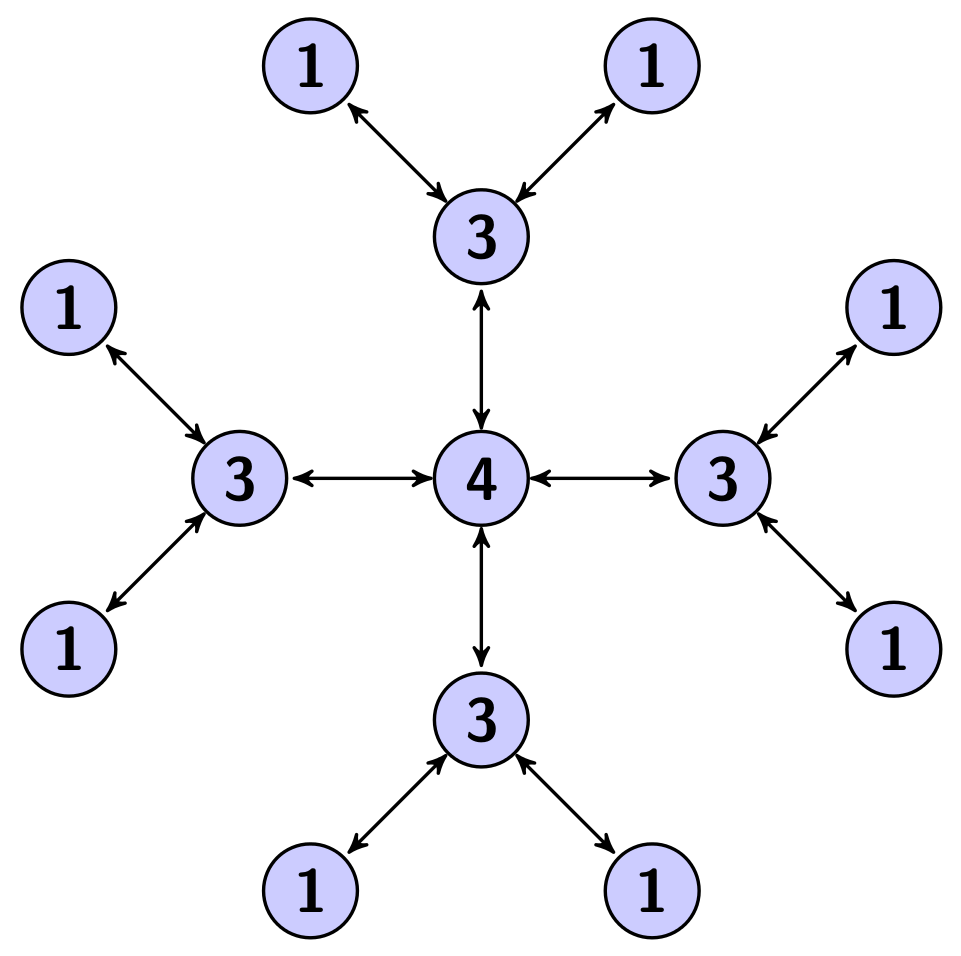
\includegraphics[scale=0.4]{imagenes/maloGreedy.png}
% 	\caption{}
%	\label{GrafoCompleto}
   \end{center}
 \end{figure}

En este ejemplo, el greedy tomará como primer nodo, al nodo del centro, y eliminará a todos sus adyacentes. Luego, tomará todas las componentes conexas restantes.
El resultado final será una solución con $(m-2)*m$ versus $m$ de la solución óptima, con $m$ igual al grado del nodo central.

Otro caso donde fallará, en la mayoría de los casos, es en los ciclos simples. Dado que estos son $2-regulares$, el orden en el que el greedy tomará los nodos, no puede ser determinado antes de su ejecución. Sólo tendrá éxito en encontrar la solución óptima, si ordena los nodos de manera tal que $\forall v_{i} \in V$, el arreglo a recorrer sea $[v_{1},...,v_{n}]$, donde $(v_{i},v_{i+1}) \in E$.

Alternativamente, el greedy siempre encontrará la solución óptima para los grafos completos y los grafos $0-regulares$ (pues la misma es trivial); pero más interesante aún, siempre encontrará la solución óptima para los grafos bipartitos completos (en los que la misma, es la partición más pequeña del bipartito).
%Describir instancias de CIDM para las cuales la heuristica no proporciona una solucion optima. Indicar que tan mala puede ser la solucion obtenida respecto de la solucion optima.

\newpage
\subsection{Experimentaci\'on}
%Realizar una experimentacion que permita observar la performance del algoritmo en terminos de tiempo de ejecucion en funcion de los parametros de la entrada.
Para la experimentación, se realizaron experimentos sobre grafos generados de manera aleatoria, fijando nodos y variando ejes, y viceversa.\\

A continuación se adjuntan los gráficos con los resultados:

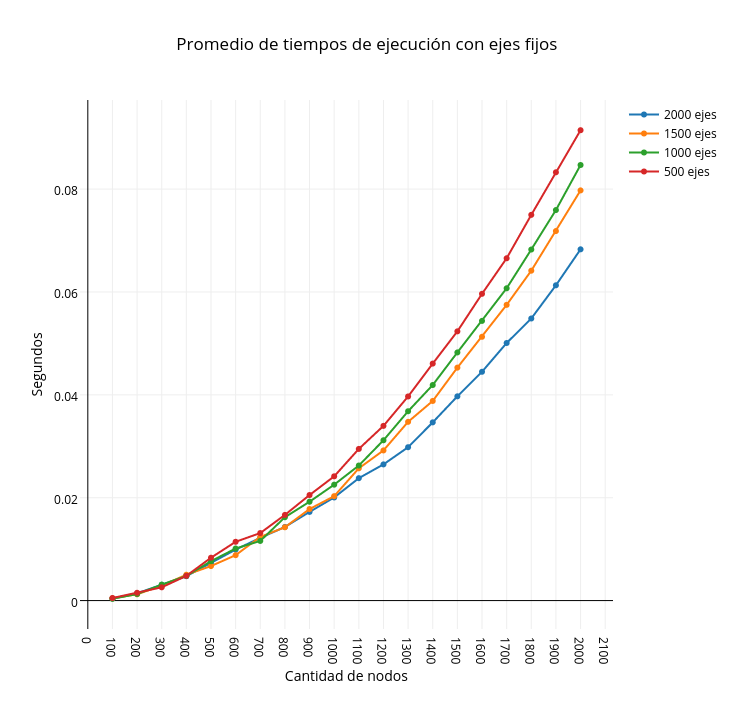
\includegraphics[width=15cm,keepaspectratio=yes]{imagenes/greedy/fixedge.png}

Como se puede observar, los tiempos aumentan a medida que disminuyen la cantidad de ejes. Esto se debe a que a menor cantidad de ejes, menor cantidad de nodos se eliminan de la lista de nodos que itera el algoritmo.

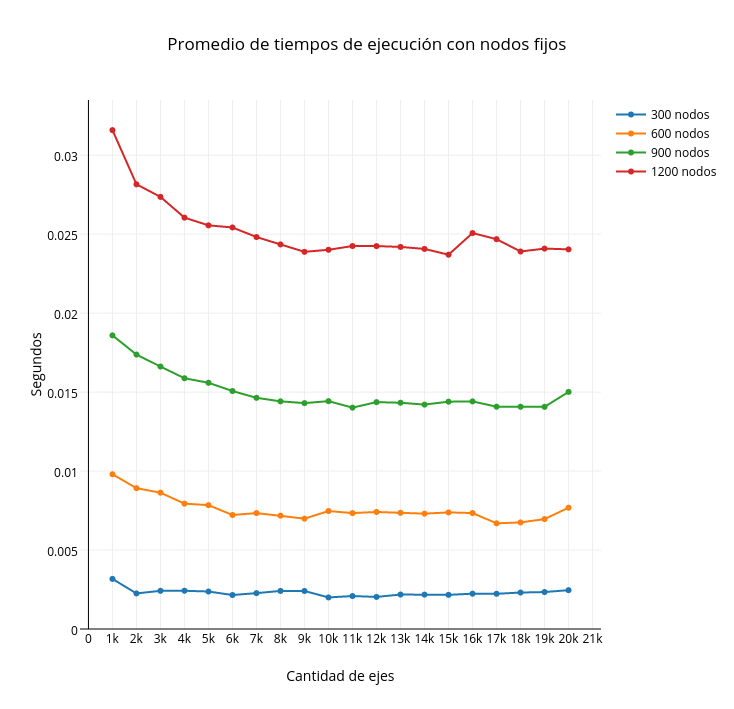
\includegraphics[width=15cm,keepaspectratio=yes]{imagenes/greedy/fixnode.png}

En este gráfico, se puede ver que si bien la cantidad de ejes (como fue mencionado en el gráfico anterior) afecta los tiempos, a mayor cantidad de ejes se puede observar que el verdadero limitante es la cantidad de nodos. Aquí se aprecia que la complejidad teórica se corresponde, en cuanto a que depende de la cantidad de nodos, y no de la cantidad de ejes.

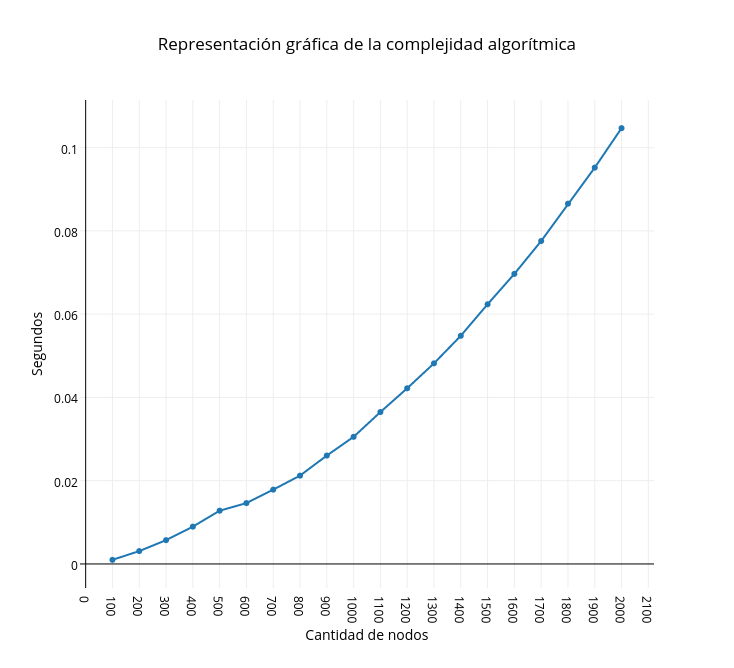
\includegraphics[width=15cm,keepaspectratio=yes]{imagenes/greedy/worst1.png}

Resultó interesante graficar, a su vez, algún caso en el que se refleje la complejidad algorítmica.
Para ello, se tomo el grafo sin ejes, es decir, todas componentes conexas, puesto que el algoritmo deberá recorrer, por cada nodo, el resto de todos los nodos preguntando si son vecinos.
Aquí se puede apreciar que efectivamente, los tiempos incrementan de manera cuadrática.

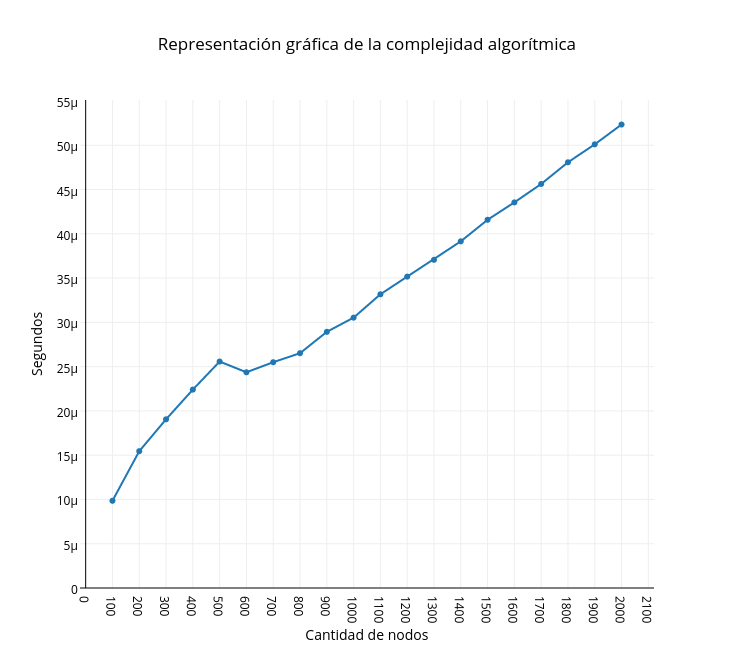
\includegraphics[width=15cm,keepaspectratio=yes]{imagenes/greedy/worst2.png}

Para asegurarnos de que efectivamente la función corresponde a la familia de funciones cuadráticas y no a otra, se procedió a dividir los resultados por el tamaño de la entrada.
Se puede apreciar que el gráfico se aproxima a una función lineal.

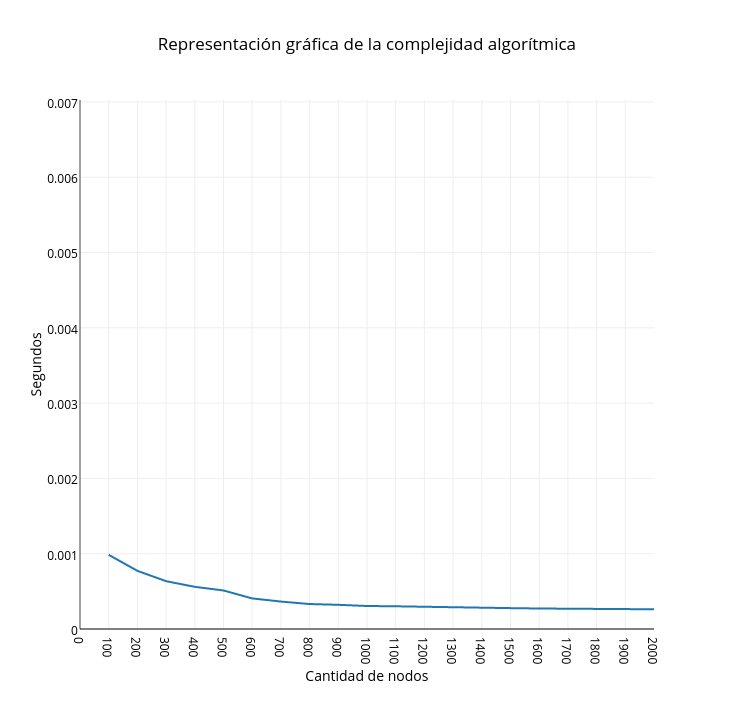
\includegraphics[width=15cm,keepaspectratio=yes]{imagenes/greedy/worst3.png}

Finalmente, se procedió a dividir los resultados (ya divididos) por el tamaño de la entrada nuevamente.
Efectivamente, el resultado tiende a una constante, lo que termina demostrando de manera empírica, la complejidad teórica explicada.
